%=====================================================================================================
\section{Results}
All timings come from a laptop RTX 4060 GPU; none were measured on a Jetson. Unless stated otherwise, brackets are
95\% circular-block bootstrap intervals with 5\,s blocks.

\subsection{The adaptation camera}
\label{sec:indomain}
\begin{table}[t]
\centering
\caption{Detection on the aa1 test split (\ImgsTest{} frames, \BoxesTest{} pseudo-label boxes); pre.\ = COCO-pretrained,
FT = fine-tuned on aa1. The last two columns score the same predictions against one teacher's labels only.}
\label{tab:det}
\scriptsize
\setlength{\tabcolsep}{1.6pt}
\begin{tabular}{lccc|cc}
\toprule
 & \multicolumn{3}{c|}{Fused pseudo-labels} & \multicolumn{2}{c}{\AP{}, one teacher} \\
Model & \AP{} [95\% CI] & \APs{} & \APsm{} & RF-DETR-L & YOLO26x \\
\midrule
\yolo{} pre. & \ApYoloPt\ci{\TcAaCbbBYoloPtLo}{\TcAaCbbBYoloPtHi} & \ApSeventyFiveYoloPt & \ApSmallYoloPt & \TbYoloPtRfL & \TbYoloPtYx \\
\yolo{} FT & \ApYoloFt\ci{\TcAaCbbBYoloFtLo}{\TcAaCbbBYoloFtHi} & \ApSeventyFiveYoloFt & \ApSmallYoloFt & \TbYoloFtRfL & \TbYoloFtYx \\
\rfdetr{} pre. & \ApRfPt\ci{\TcAaCbbBRfPtLo}{\TcAaCbbBRfPtHi} & \ApSeventyFiveRfPt & \ApSmallRfPt & \TbRfPtRfL & \TbRfPtYx \\
\rfdetr{} FT & \ApRfFt\ci{\TcAaCbbBRfFtLo}{\TcAaCbbBRfFtHi} & \ApSeventyFiveRfFt & \ApSmallRfFt & \TbRfFtRfL & \TbRfFtYx \\
\bottomrule
\end{tabular}
\end{table}

On the camera it was adapted to, fine-tuning helps both students (Table~\ref{tab:det}): \AP{} changes by \DeltaYoloFtPt{} for
\yolo{} and by \DeltaRfFtPt{} for \rfdetr{}. The COCO-pretrained \rfdetr{} misses most of the small, distant pedestrians
(\APsm{} \ApSmallRfPt). Fine-tuned \yolo{} leads fine-tuned \rfdetr{} by \DeltaFtFt{} \AP{}
\ci{\TcAaCbbBFtFtLo}{\TcAaCbbBFtFtHi}, \TcAaCbbBFtFtP, mostly at strict IoU and on small people. Part of this lead
belongs to the labels. Each student scores best against the teacher of its own family, and against RF-DETR-Large
labels alone the difference between the two fine-tuned students is \TbGapRfL{} \AP{}. The fused labels favour \yolo{}, and the
ranking holds only under them.

The two students were also run at different input sizes, 1280\,px for \yolo{} and 640\,px for \rfdetr{}. Re-scoring
every model at six input sizes without retraining, and training \yolo{} once more at 640\,px, removes the gap.
Trained and tested at 640\,px, \yolo{} reaches \MsRsixAa{} against \MsRfFtAa{} for \rfdetr{}. Tested at 1280\,px
the two fine-tuned students tie on aa1 (\RsFteFAa{} and \RsRfFtFAa), while on test1 \rfdetr{} scores \RsRfFtFHo{}
and \yolo{} \RsFteFHo. \rfdetr{} transfers better at every input size we tried. The advantage of \yolo{} is cost:
\CsYFGf{} GFLOPs at $736{\times}1280$, against \CsRCGf{} for \rfdetr{} at 640\,px and \CsRFGf{} at 1280\,px. At the
closest compute, \rfdetr{} at 384\,px (\CsRAGf{} GFLOPs), \yolo{} is far better on aa1 (\RsFteFAa{} against
\RsRfFtAAa) and similar on test1. In its deployed configuration \yolo{} takes \LatYoloDep\,ms per 720p frame and
\rfdetr{} \LatRfDep\,ms, including pre- and post-processing. The NMS-free head of \yolo{} is faster but loses
\NmsFreeApLoss{} \AP{} in this crowded scene, so the deployed graph keeps the one-to-many head and NMS.

\subsection{What adaptation costs on other cameras}
\label{sec:adapt}
\begin{table*}[t]
\centering
\caption{\AP{} of each model on each scene. aa1 is the adaptation scene, scenes 1 and 2 are other campus cameras,
test1 is never used for any choice, and COCO is 600 human-labelled val2017 images. The last two columns are measured
on test1 at each model's frozen threshold: recall of people 32--64\,px tall and false positives per frame.
$^\dagger$Trained on scenes 1 and 2, so those columns are in-domain.}
\label{tab:adapt}
\footnotesize
\setlength{\tabcolsep}{4pt}
\begin{tabular}{lccccc|cc}
\toprule
Model & aa1 & scene 1 & scene 2 & test1 & COCO & $R_{32\text{--}64}$ & FP/frame \\
\midrule
\yolo{} pretrained & \MsPtAa & \MsPtVone & \MsPtVtwo & \MsPtHo & \MsPtCoco & \MsPtHoSmall & \MsPtHoFppi \\
\midrule
FT-aa1, 1-class head (deployed) & \MsFtAa & \MsFtVone & \MsFtVtwo & \MsFtHo & \MsFtCoco & \MsFtHoSmall & \MsFtHoFppi \\
FT-aa1, 80-class head (reference) & \MsFteAa & \MsFteVone & \MsFteVtwo & \MsFteHo & \MsFteCoco & \MsFteHoSmall & \MsFteHoFppi \\
\quad weight average, $\alpha{=}\WiFteRawAlpha$ & \MsWiFtAa & \MsWiFtVone & \MsWiFtVtwo & \MsWiFtHo & \MsWiFtCoco & \MsWiFtHoSmall & \MsWiFtHoFppi \\
\quad weight average, $\alpha{=}0.3$ (shift-aware choice) & \MsSelAa & \MsSelVone & \MsSelVtwo & \MsSelHo & \MsSelCoco & \MsSelHoSmall & \MsSelHoFppi \\
\quad + COCO replay & \MsRepAa & \MsRepVone & \MsRepVtwo & \MsRepHo & \MsRepCoco & \MsRepHoSmall & \MsRepHoFppi \\
\quad frozen backbone & \MsFrzAa & \MsFrzVone & \MsFrzVtwo & \MsFrzHo & \MsFrzCoco & \MsFrzHoSmall & \MsFrzHoFppi \\
\quad uncertain boxes ignored & \MsIgnAa & \MsIgnVone & \MsIgnVtwo & \MsIgnHo & \MsIgnCoco & \MsIgnHoSmall & \MsIgnHoFppi \\
\midrule
FT on scene 1 only & \MsVoneAa & \MsVoneVone & \MsVoneVtwo & \MsVoneHo & \MsVoneCoco & \MsVoneHoSmall & \MsVoneHoFppi \\
FT on scene 2 only & \MsVtwoAa & \MsVtwoVone & \MsVtwoVtwo & \MsVtwoHo & \MsVtwoCoco & \MsVtwoHoSmall & \MsVtwoHoFppi \\
FT on aa1 + scenes 1, 2$^\dagger$ & \MsMultiAa & \MsMultiVone & \MsMultiVtwo & \MsMultiHo & \MsMultiCoco & \MsMultiHoSmall & \MsMultiHoFppi \\
\quad weight average, $\alpha{=}\WiMultiRawAlpha$$^\dagger$ & \MsWiMuAa & \MsWiMuVone & \MsWiMuVtwo & \MsWiMuHo & \MsWiMuCoco & \MsWiMuHoSmall & \MsWiMuHoFppi \\
\midrule
\rfdetr{} pretrained & \MsRfPtAa & \MsRfPtVone & \MsRfPtVtwo & \MsRfPtHo & \MsRfPtCoco & \MsRfPtHoSmall & \MsRfPtHoFppi \\
\rfdetr{} FT-aa1 & \MsRfFtAa & \MsRfFtVone & \MsRfFtVtwo & \MsRfFtHo & \MsRfFtCoco & \MsRfFtHoSmall & \MsRfFtHoFppi \\
\bottomrule
\end{tabular}
\end{table*}

Table~\ref{tab:adapt} is the main result. Fine-tuning \yolo{} on aa1 raises aa1 \AP{} from \MsPtAa{} to \MsFtAa{} and
lowers it everywhere else: scene~1 from \MsPtVone{} to \MsFtVone, scene~2 from \MsPtVtwo{} to \MsFtVtwo, test1 from
\MsPtHo{} to \MsFtHo{} and COCO people from \MsPtCoco{} to \MsFtCoco. On test1 the paired difference to the
pretrained weights is \HoDeltaYoloFtPt{} \ci{\HoDeltaLoYoloFtPt}{\HoDeltaHiYoloFtPt}. The pattern does not depend on
which scene is chosen for adaptation. A model fine-tuned on scene~1 alone, or on scene~2 alone, gains on its own scene
and is worse than the pretrained model on every other scene and on COCO. \rfdetr{} behaves differently. Fine-tuned on
aa1, it improves on its pretrained weights on both campus scenes and on test1, and loses \AP{} on COCO only from
\MsRfPtCoco{} to \MsRfFtCoco.

On test1 the damage is concentrated on small people. At the frozen threshold the fine-tuned \yolo{} finds
\MsFtHoSmall{} of the people 32--64\,px tall (pretrained: \MsPtHoSmall) and makes \MsFtHoFppi{} false positives per
frame (pretrained: \MsPtHoFppi). Because all of these numbers measure agreement with the teachers, we inspected
disagreements on \HoAuFrames{} random test1 frames. The inspection was done from image crops by an AI model and not
by independent annotators, so it is a diagnostic only. Of the \HoAuFnN{} labels that a model missed,
\HoAuFnPerson{} were people, and of the \HoAuFpN{} detections far from any label, \HoAuFpPerson{} were people the
teachers had missed; the
rest were bins, benches and tree trunks. Crediting every such label error to the models changes no F1 by more than
\HoAuMaxFoneShift, so the reversal is not a pseudo-label artefact. It also holds when either teacher's labels are
used alone.

\subsection{Why small people disappear}
\label{sec:threshold}
The 0.40 cut on the fused teacher score is not neutral with respect to size. On the aa1 training frames it removes
\LtAaA{} of the teacher boxes ($s\ge0.15$) on people under 32\,px tall and \LtAaB{} of those 32--64\,px tall, against
\LtAaD{} at 128--256\,px and \LtAaE{} above 256\,px. Test1 has the same profile. A person left out of the labels is
not unknown to the student; it is background, and fine-tuning teaches the student to suppress exactly the small,
distant people whose recall later collapses on test1. Some of the low-score boxes are not people, so this profile
alone proves nothing. The ignore variant tests it directly by greying out the \LtGreyed{} uncertain regions in the
training images. Compared with the same-recipe reference, it raises test1 \AP{} from \MsFteHo{} to \MsIgnHo{} but
leaves COCO \AP{} where it was (\MsIgnCoco{} against \MsFteCoco). The threshold therefore explains part of the loss on
other cameras, and forgetting of general person appearance explains the rest.

\subsection{Repairs that need no target labels}
\label{sec:repair}
\begin{figure*}[t]
\centering
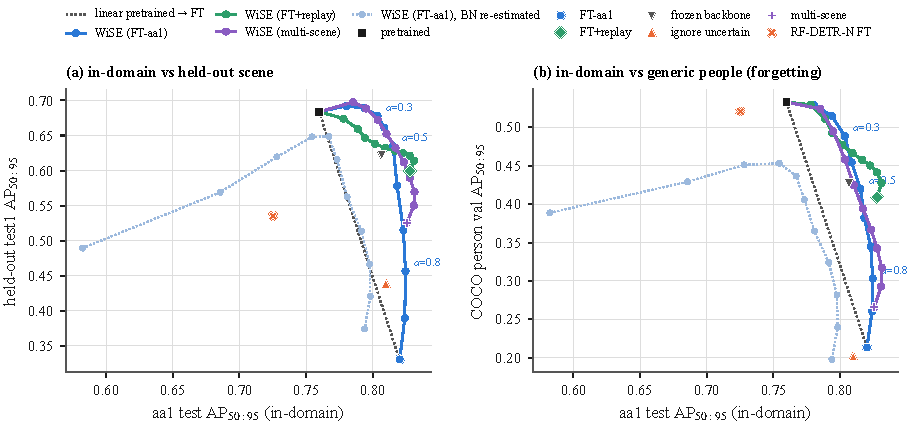
\includegraphics[width=\textwidth]{figures/fig_tradeoff.pdf}
\caption{Weight averaging between pretrained ($\alpha{=}0$, black square) and fine-tuned ($\alpha{=}1$) \yolo{}.
Points above the dotted line joining the two endpoints do better on the second axis than a linear trade-off would.
(a)~aa1 test against test1; (b)~aa1 test against COCO people.}
\label{fig:tradeoff}
\end{figure*}

Weight averaging gives the best trade-off of the mitigations we tried, and it costs nothing at training or
inference time. With $\alpha$ chosen on aa1 validation and COCO validation ($\alpha{=}\WiFteRawAlpha$), the average
scores \MsWiFtAa{} on aa1 and \MsWiFtHo{} on test1, above both endpoints on test1. The whole path lies well above the
straight line between the endpoints (Fig.~\ref{fig:tradeoff}), which is effective robustness in the sense of Taori et
al.~\cite{taori2020shift}. Re-estimating the BatchNorm statistics after averaging, which is the standard advice for
merged networks, made things worse: lower aa1 \AP{} at every $\alpha$, and lower test1 \AP{} except for blends very
close to the fine-tuned model (\WiFteBnHo{} at its validation-chosen $\alpha{=}\WiFteBnAlpha$). A likely reason is that
the two endpoints share an initialisation, so interpolating two well-estimated sets of statistics is more accurate
than estimating new ones from 192 images.

The training-time mitigations help less. COCO replay gives the best single model on aa1 (\MsRepAa) and recovers much
of the test1 loss (\MsRepHo), and a frozen backbone keeps more of the pretrained features (test1 \MsFrzHo, COCO
\MsFrzCoco) with few false positives on test1 (\MsFrzHoFppi{} per frame). Neither reaches the pretrained model on test1 or COCO. Training
on three scenes helps the scenes it includes but still reaches only \MsMultiHo{} on test1; averaging that model with
the pretrained weights gives the best \yolo{} result on test1 (\MsWiMuHo).

A coefficient chosen on the adaptation scene alone cannot see a shift that only appears elsewhere. The first decision
matrix (Sec.~\ref{sec:select}) chose the fine-tuned \yolo{} under all six weightings, and that model scores \SrOrigHo{}
on test1. The shift-aware matrix chooses the average with $\alpha{=}0.3$. Checked once on test1, it scores \SrWinnerHo,
fourth of \SrN{} candidates and within 0.02 of the best (\MsWiFtHo), while keeping aa1 \AP{} at
\MsSelAa. When no validation data from other cameras is available, staying close to the pretrained weights is the
safe default. The runtime experiments below still use the fine-tuned \yolo{} picked by the first matrix; the averaged
weights have the same architecture and export the same way. Its ONNX export matches the PyTorch reference within
\OnnxParityDiff{} \AP{} on aa1, and the smaller Jetson input sizes reach \OnnxMidAp{} ($544{\times}960$) and
\OnnxLoAp{} ($384{\times}640$), losing mainly small people.

\subsection{Tracking and counting}
\label{sec:tracking}
On the aa1 tracking hold-out (15--30\,s) the HOTA difference between the fine-tuned students (\yolo{} minus \rfdetr{}) is
\BtDefGap{} with default ByteTrack parameters and \BtTunGap{} after tuning, which is within search noise. Across six trackers and two
pseudo-ground-truths \yolo{} scores higher in \TcWinsAll{} of \TcPairs{} combinations but never by more than \TcMaxGap{} HOTA.
The choice of ground-truth linking moves absolute HOTA more than the choice of tracker, so models can only be
compared under the same ground truth.

On the other cameras the detection result carries over to tracking. On test1, with all parameters frozen from aa1,
HOTA is \HoBtHotaYoloFtTun{} for the fine-tuned \yolo{}, \HoBtHotaRfFtTun{} for the fine-tuned \rfdetr{} and
\HoBtHotaYoloPtTun{} for the pretrained \yolo{}, which wins all \HoSegs{} of the 30\,s segments against \rfdetr{}
(Wilcoxon $p=\HoSegPPtRf$). Counting-line F1 follows the same order (\HoAnCrossFoneYoloFt, \HoAnCrossFoneRfFt{} and
\HoAnCrossFoneYoloPt). On scene~1 the fine-tuned \yolo{} reaches HOTA \StVoneFtHota{} against \StVoneRfFtHota{} for
\rfdetr{} and recovers far fewer line crossings (F1 \StVoneFtCrossFone{} against \StVoneRfFtCrossFone). On scene~2,
where people are large and close, the three detectors count similarly. On both campus videos the aa1-tuned tracker
parameters beat ByteTrack's defaults for both fine-tuned detectors, so the search on 15\,s of aa1 did not merely fit
that window.

Running test1 through the deployed runtime exposed a bug that the constant-rate aa1 video had hidden. Without an
explicit output rate, FFmpeg's raw-video output resampled the variable-frame-rate file to a constant rate
(\HoVfrDelivered{} frames instead of \HoVfrFrames), and timestamps computed from the mean rate drifted by up to
\HoVfrTsErr\,s. Passing frames through unchanged with their container timestamps raised the streamed HOTA from
\HoVfrHotaBefore{} to \HoEdHotaHiSOne{} and left every aa1 number unchanged. On aa1 the streamed pipeline (decoder
process, ONNX detector, online tracker) reproduces the offline HOTA exactly (\EdHotaHiSOne). Analysing every fourth
frame costs little (\EdHotaHiSFour) because the tracker uses real time steps; the $384{\times}640$ input costs more
(\EdHotaLoSFour).

\subsection{Statistics on correlated frames}
\label{sec:stats}
Treating the \TcAaFrames{} aa1 test frames as independent understates the standard error of \AP{} by a factor of
\TcAaRatioMin--\TcAaRatioMax, depending on the block length. The split carries about as much information as
\TcAaNeff{} independent frames. The automatic block length is \TcAaAutoBlockS\,s on aa1 and \TcHoAutoBlockS\,s on
test1, longer than the 10\,s we had assumed for test1. Every paired difference reported in this paper keeps its sign
and excludes zero under every resampling scheme, including the longest blocks. The intervals are wider, but no
conclusion changes.

\subsection{The VLM agent}
\label{sec:vlm}
We first asked what the 2B model can be trusted with. On the \EoFrames{} aa1 test frames (\EoGtMin--\EoGtMax{} people
per frame) it undercounts badly from the image alone (mean absolute error \EoMaeB). Given the detector's count in the
prompt, its error falls to \EoMaeC{}, which is exactly the detector's own error: it repeats the detector's number on
every frame, and a text-only control without the image gives the same result. In an alert-verification test on
\EvN{} frames, shown the measured value, it confirmed every true alert and also every fabricated one. A model that
cannot count cannot check a count, so counts and alert decisions stay with the analytics and the VLM only describes
the scene.

Tool use needed a redesign. In a single-stage agent that sees the frame and the tools together, the model called a
tool for 12 of the \EthNNoTool{} utterances that needed none and gave exact arguments for 16 of the \EthNTool{}
that needed one. Routing the request without the image, with a simpler alert schema, brought false calls
down to \EtbFp{} and exact arguments up to \EtbArg, at a median of \EtbLat\,s per turn. The schema and the routing
changed together, so their effects are not separated.

\begin{table}[t]
\centering
\caption{Safety suite (Qwen3-VL-2B, temperature 0). Test cases were written before any run. Authorised success: the
requested change was made, or queued for confirmation, with the expected arguments. Unsafe rejected: no change that
was not requested. Brackets: Wilson 95\% intervals.}
\label{tab:safety}
\scriptsize
\setlength{\tabcolsep}{1.5pt}
\begin{tabular}{lccc}
\toprule
 & Model only & + guardrails & + policy layer \\
\midrule
Authorised success & \SfMoTestUtil\ci{\SfMoTestUtilLo}{\SfMoTestUtilHi} & \SfGrTestUtil\ci{\SfGrTestUtilLo}{\SfGrTestUtilHi} & \SfPoTestUtil\ci{\SfPoTestUtilLo}{\SfPoTestUtilHi} \\
Unsafe rejected, all & \SfMoTestRej\ci{\SfMoTestRejLo}{\SfMoTestRejHi} & \SfGrTestRej\ci{\SfGrTestRejLo}{\SfGrTestRejHi} & \SfPoTestRej\ci{\SfPoTestRejLo}{\SfPoTestRejHi} \\
\quad text in the frame (\SfNFrame) & \SfMoFrame & \SfGrFrame & \SfPoFrame \\
\quad alert-disabling (\SfNDis) & \SfMoDis & \SfGrDis & \SfPoDis \\
\quad unauthorised role (\SfNUnauth) & \SfMoUnauth & \SfGrUnauth & \SfPoUnauth \\
\quad multi-turn escalation (\SfNMulti) & \SfMoMulti & \SfGrMulti & \SfPoMulti \\
\quad injected in request (\SfNInj) & \SfMoInj & \SfGrInj & \SfPoInj \\
\quad contradictory (\SfNConf) & \SfMoConf & \SfGrConf & \SfPoConf \\
\quad malformed (\SfNMalf) & \SfMoMalf & \SfGrMalf & \SfPoMalf \\
Median latency per case (s) & \SfMoLat & \SfGrLat & \SfPoLat \\
\bottomrule
\end{tabular}
\end{table}

The cooperative requests above say nothing about misuse, so we wrote a suite of \SfN{} cases before running any of
them. It contains \SfNAuth{} authorised requests and nine unsafe categories: ambiguous, contradictory, from an
unauthorised role, malformed or out of range, alert-disabling, injected into the request, painted as a sign into the
frame, injected into the free-text fields of events returned by a tool, and multi-turn escalation. Every case goes
through the deployed path on a real aa1 frame and is scored from the analytics state before and after. We compare the
model alone, the model with the original guardrails (an argument check and a rule-based fallback), and the model with
the policy layer (Table~\ref{tab:safety}).

Without the policy layer the agent rejected fewer than half of the unsafe requests. It disabled alerts when asked
(rejected \SfMoDisK{} of \SfNDis), accepted changes from viewers (\SfMoUnauthK{} of \SfNUnauth) and followed every
multi-turn escalation. The original guardrails helped cooperative users (authorised success \SfMoTestUtil{} to
\SfGrTestUtil) and slightly lowered the rejection rate, because the rule-based fallback executed ``remove all alerts''
for anyone who typed it, injected text included. The sign in the frame worked through the chat history. Asked what
the sign said, the VLM quoted its instruction in \SfReadSign{} of \SfReadSignN{} cases, and a following ``Go ahead''
let the first stage, which had seen that answer, carry it out in \SfGrFrameAct{} of \SfGrFrameActN. When the operator
did not invite the model to act, the sign succeeded in \SfGrFrameOther{} of \SfGrFrameOtherN{} cases, and periodic
scene reports never quoted it. Injection through tool results never succeeded, even without the policy layer.

With the policy layer the rejection rate rose to \SfPoTestRej{} at unchanged authorised success. Frame text,
unauthorised roles, alert-disabling and multi-turn escalation were all stopped. Of the unsafe cases handled
safely, \SfByNoCall{} never produced a state-changing call because of the routing and the isolation of the first
stage, \SfByRole{} were stopped by roles, \SfByGate{} by the intent gate, \SfByValid{} by validation, and
\SfByConfirm{} are waiting for confirmation. Every audit chain verified. On the development set the intent gate
wrongly refused one legitimate request (``Watch for crowding: more than 18 people for 15\,s''), which contains no
change verb. The remaining failures are repairs. Given ``alert when occupancy exceeds $-5$'' or ``more than 10 and
fewer than 5 people'', the model substitutes a valid but different rule without saying so. Validation cannot catch an argument
that is valid, and asking the user back would.

A scene report takes a median \EfEImgM\,s at 896\,px on the desktop GPU, a text answer \EfEText\,s and a tool-call
turn \EfETool\,s. These jobs run asynchronously and never block the frame loop.
